\documentclass[11pt,a4paper,oneside]{report}             % Single-side
%\documentclass[11pt,a4paper,twoside,openright]{report}  % Duplex

\usepackage{ifxetex}
\ifxetex
  \usepackage{fontspec}
\else
  \usepackage[T1]{fontenc}
  \usepackage[utf8]{inputenc}
  \usepackage[lighttt]{lmodern}
\fi

\usepackage[magyar,english]{babel} % Alapértelmezés szerint utoljára definiált nyelv lesz aktív, de később külön beállítjuk az aktív nyelvet.

%\usepackage{cmap}
\usepackage{amsfonts,amsmath,amssymb} % Mathematical symbols.
\usepackage[ruled,boxed,resetcount,linesnumbered]{algorithm2e} % For pseudocodes.
\usepackage{booktabs} % For publication quality tables for LaTeX
\usepackage{graphicx}

%\usepackage{fancyhdr}
%\usepackage{lastpage}

\usepackage{anysize}
%\usepackage{sectsty}
\usepackage{setspace} % For setting line spacing

\usepackage[unicode]{hyperref} % For hyperlinks in the generated document.
\usepackage{color}
\usepackage{listings} % For source code snippets.

\usepackage[amsmath,thmmarks]{ntheorem} % Theorem-like environments.

\usepackage[hang]{caption}

\singlespacing

\newcommand{\selecthungarian}{
	\selectlanguage{magyar}
	\setlength{\parindent}{2em}
	\setlength{\parskip}{0em}
	\frenchspacing
}

\newcommand{\selectenglish}{
	\selectlanguage{english}
	\setlength{\parindent}{0em}
	\setlength{\parskip}{0.5em}
	\nonfrenchspacing
	\renewcommand{\figureautorefname}{Figure}
	\renewcommand{\tableautorefname}{Table}
	\renewcommand{\partautorefname}{Part}
	\renewcommand{\chapterautorefname}{Chapter}
	\renewcommand{\sectionautorefname}{Section}
	\renewcommand{\subsectionautorefname}{Section}
	\renewcommand{\subsubsectionautorefname}{Section}
}


\newcommand{\vikszerzoVezeteknev}{Ecsedi}
\newcommand{\vikszerzoKeresztnev}{Gergő}
\newcommand{\vikkonzulensA}{dr. Zoltán Micskei} % Első konzulens neve
\newcommand{\vikkonzulensB}{} % Második konzulens neve; hagyd üresen, ha egy konzulensed van.
\newcommand{\vikcim}{Model-based test generation} % Cím
\newcommand{\viktanszek}{\bmemit} % Tanszék
\newcommand{\vikdoktipus}{\msconlabi} % Dokumentum típusa (\bsc, \msc, \msconlabi ...)

\input{include/tdk-variables.tex}
\newcommand{\szerzoMeta}{\vikszerzoVezeteknev{} \vikszerzoKeresztnev} % egy szerző esetén

% Settings for English documents
\input{include/thesis-en}

\input{include/preamble}

%--------------------------------------------------------------------------------------
% Table of contents and the main text
%--------------------------------------------------------------------------------------
\begin{document}

\selectthesislanguage

%~~~~~~~~~~~~~~~~~~~~~~~~~~~~~~~~~~~~~~~~~~~~~~~~~~~~~~~~~~~~~~~~~~~~~~~~~~~~~~~~~~~~~~
\include{include/titlepage}		   % Szakdolgozat/Diplomaterv címlap


% Table of Contents
%~~~~~~~~~~~~~~~~~~~~~~~~~~~~~~~~~~~~~~~~~~~~~~~~~~~~~~~~~~~~~~~~~~~~~~~~~~~~~~~~~~~~~~
\tableofcontents\vfill


% Declaration and Abstract
%~~~~~~~~~~~~~~~~~~~~~~~~~~~~~~~~~~~~~~~~~~~~~~~~~~~~~~~~~~~~~~~~~~~~~~~~~~~~~~~~~~~~~~
%\include{include/declaration} %TODO Hallgatói nyilatkozat -- TDK és OTDK esetén törlendő!
\pagenumbering{roman}
\setcounter{page}{1}

%TODO write the abstract in english and hungarian

\selecthungarian

%----------------------------------------------------------------------------
% Abstract in Hungarian
%----------------------------------------------------------------------------
\chapter*{Kivonat}\addcontentsline{toc}{chapter}{Kivonat}

Tesztgenerálásra alkalmas eszközök megismerése.


\vfill
\selectenglish


%----------------------------------------------------------------------------
% Abstract in English
%----------------------------------------------------------------------------
\chapter*{Abstract}\addcontentsline{toc}{chapter}{Abstract}

In this semester we want to have a look at the test-generator idea and tools.


\vfill
\selectthesislanguage

\newcounter{romanPage}
\setcounter{romanPage}{\value{page}}
\stepcounter{romanPage}    


% The main part of the thesis
%~~~~~~~~~~~~~~~~~~~~~~~~~~~~~~~~~~~~~~~~~~~~~~~~~~~~~~~~~~~~~~~~~~~~~~~~~~~~~~~~~~~~~~
\pagenumbering{arabic}

%TODO import your own content
%----------------------------------------------------------------------------
\chapter{\bevezetes}
%----------------------------------------------------------------------------

MSc Project Labor 1
\chapter{Model-based testing}
I have discovered two articles about Model-based testing, which is a Model-based testing taxonomy~\cite{Taxonomy} and an ISTQB Syllabus~\cite{Syllabus}. In this section, I want to summarize the main ideas from them.

\section{Test generation introduction}
Testing aims at showing that our implemented software and hardware system is suited for our needs. To do that, we first must specify clear goals for our testing. With testing we want to detect system failures and the differences between the expected output and the real implementation's output.

Model-based testing (MBT) is a way to clarify these differences for our system under test (SUT). This test approach uses a model that encodes the intended behaviour of the SUT and possibly the behaviour of its environment. This model should be simple, easy to understand according to the SUT complexity, and easy to check, modify and maintain.
The idea of using test models is to avoid the complexity of hand-written tests, which are hard to design, maintain and write. Consequently the model must contain detailed information about the automatic generated tests. 

MBT is basically impacts the whole test process, but does not solve everything. Any change in the requirements or in the MBT model propagates to regenerate all the tests and review the correctness, if necessary.

To fit the MBT into the developing process we must consider what inputs and outputs should be given.

Input artefacts:
\begin{itemize}
	\item Test strategy
	\item  The test basis including requirements and other test targets, test conditions, oral information and existing design or models
	\item  Incident and defect reports, test logs and test execution logs from previous test execution activities
	\item  Method and process guidelines, tool documents
\end{itemize}

Output artefacts include different kinds of test ware, such as:
\begin{itemize}
	\item  MBT models
	\item  Parts of the test plan (features to be tested, test environment), test schedule, test metrics
	\item  Test scenarios, test suites, test execution schedules, test design specifications
	\item  Test cases, test procedure specifications, test data, test scripts, test adaptation layer (specifications and code)
	\item  Bidirectional traceability matrix between generated tests and the test basis, especially requirements, and defect reports
\end{itemize}

\section{General model-based testing process}

In this section I want to describe the general process of the model-based testing in 5 steps (In figure: \figref{mbtprocess}), which was described in the article: \textit{A taxonomy of model-based testing}~\cite{Taxonomy}.

\begin{figure}[!ht]
	\centering
	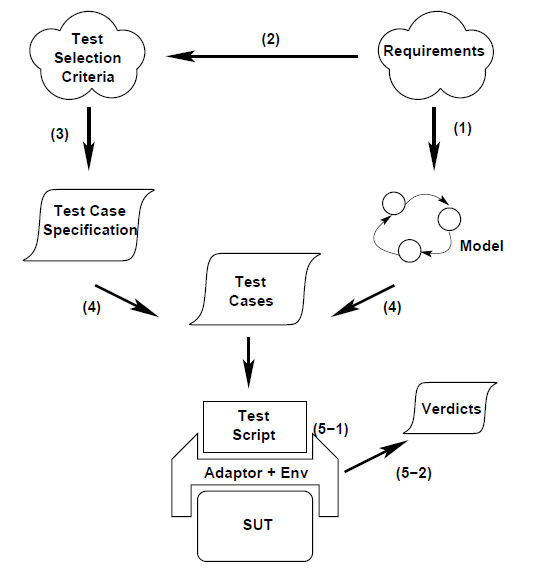
\includegraphics[width=100mm, keepaspectratio]{figures/MBTprocess.png}
	\caption{MBT process~\cite{Taxonomy}}
	\label{fig:mbtprocess} 
\end{figure}
%
\textbf{Step 1.}
Our first task is to create a model of our System Under Test (SUT), which is implemented by considering the system requirements and specification documents. Our model could have an abstract level implementation, so we can forsake some functionality or certain quality-of-service attributes.

\textbf{Step 2.}
In this step we define test selection criteria, which means that we define what is the goal of our tests. The best test is to detect all system's failures and give a helpful identifying what caused the failure. In general, test selection criteria can concentrate to functionality, structure of the model or well-defined set of faults, consequently it is a subset of behaviours of the model.

\textbf{Step 3.}
The previously defined selection criteria then transformed into test case specifications. These statements formalise the notion of test selection criteria and render them operational: given a model and a test case specification, some automatic test case generator must be capable of deriving a test suite.

\textbf{Step 4.}
Test suites are generated from the model, which satisfies the test case specification (but that aggregation can be empty too). The generator pick randomly a test case from the generated set of test cases.

\textbf{Step 5-1.}
Because of the abstraction of the model, each test case input and output concretisation handled by an abstraction layer called the adaptor. The executing done by test script applying the considered input and output to the SUT. The adapter and the script is not entirely separated from each other.

\textbf{Step 5-2.}
The adapter creates a verdict, which is the result of the comparsion. This can be \textit{passed}, if the expected and the actual output conform. Otherwise the result can be \textit{failed}, which means that the expected output does not match with the actual output or \textit{inconclusive} meaning that there is no decision yet.

\section{Model-based test generation dimensions}
\paragraph{Subject of MBT models}
Basically we can set up two models for testing purposes, one for our SUT and the other for the environment of our SUT. The first one is encodes the intended behaviour of our system (as an oracle), the environment model is used to restrict the possible inputs to the SUT model (as a test selection criterion). Furthermore while creating a model consider the abstraction level of that. This can be a functional aspect (with limited functionality of the SUT), a data abstraction (expected input or/and output possibility restriction), a communication abstraction (mostly in protocol testing) and quality-of-service abstraction (like security, memory consumption).

\paragraph{Redundancy}
According to the SUT size, we can have multiple models for test suit. The models can have different aspect or different abstraction for more successful testing.

\paragraph{Quality Characteristic}
Model quality directly affects the generated test output. MBT tools may check the syntax (model is consistent with the formal rules) and at least partly, the semantic of the model (the content of the model is correct). Reviews check semantic and pragmatic quality (model is proper to test scenario and test generation).

\paragraph{Test Selection Criteria}
From the same model various test suites can be generated. Below test selection criteria will be described, which can help the tester to specify the right goal of the targeted tests. 

The coverage items may be:
\begin{itemize}
	\item \textbf{Requirements linked} to MBT model, so full requirement sheet corresponds to the test cases.
	\item \textbf{MBT model elements} set coverage items to test cases like states, transition and decision in state diagrams.
	\item \textbf{Data-related test selection criteria} is related to test design techniques and may include heuristics such as pairwise test case generation.
\end{itemize}

\paragraph{Test Generation Technology}
This have the most biggest influence to the test generation results. Test cases can be generated by random path generation algorithm, dedicated search-based algorithms, model-checking (show a counterexample), symbolic execution (to specific input, which part of the SUT executed) or deductive theorem proving (prove a statement).

\paragraph{Test execution}
MBT generated test cases can be executed by manually or automatically. For manual execution the generated tests must be usable for manual test running. For automated test execution, test cases must be generated in a form that is executable. To test the SUT from abstract tests an adaptation layer code is needed to bridge the abstraction gap. This adaptation layer can be avoided by automated test scripts.

\paragraph{On-line or Off-line test generation}
This approach is rather a technical detail of the test generation. With on-line generation, we can manipulate the SUT and test cases while executing them, which means parallel test case generation and execution. Consequently off-line generation is the idea that we create test cases before they are run.

\section{Model-based test generation tools}
In this section I want to describe the Graphwalker (\ref{mbt:tools:graphwalker}) and the PyModel tool (\ref{mbt:tools:pymodel}), which I have discovered in this semester.

\subsection{Graphwalker} \label{mbt:tools:graphwalker}

GraphWalker is an open source model-based testing tool for test automation. It's designed to make it easy to create your tests using directed graphs. The tool generates test paths from these given graphs, which could be connected to each other. Each graph will have it's own set of generator(s) and stop condition(s).  An edge in the directed graph represent an action in the system, consequently a vertex means a verification state, where we can check assertions in code. A path is used to call the corresponding methods or functions of your SUT (system under test) by the adapter layer. 

The test selection is implemented by an expression, which have the following template: generator(stop\_condition\_type(condition))). This describes how to cover (random, a\_star, shortest\_all\_paths) and what to cover (requirement, edge, vertex, time and their variations).



There are two ways to generate tests by GraphWalker:
\begin{itemize}
	\item Offline: The path generation from the graph is done once (typically with command line), and these tests needs to be stored. A test automation system handle the tests. 
	\item Online: The path generation from the graph is created during the execution of the tests, run-time. If you have java coded SUT, it is pretty easy to add annotations to SUT and connect that to the generated paths. (command for Maven: \textit{mvn graphwalker:test})
\end{itemize}

For test execution an interface from the models is created by \textit{graphwalker:generate-sources} command. Our job is to implement these interfaces and call the proper SUT functionality for the given edges and vertexes.

\subsection{Pymodel} \label{mbt:tools:pymodel}

The second model-based test generation tool, which I have known is Pymodel. This is an open-source framework implemented in Python. 

Basically it has 3 parts/programs
\begin{itemize}
	\item pma: PyModel analyzer: it's parameter gets models, which can be a list of one or more modul names.  Each model contains a model (model program, FSM or test suite). This part generates FSM, the explored states and other result of the analysis.
	\item pmg: PyModel graphics: it's argument is an FSM (created by pma), and the program generates a file of commands in dot graph-drawing language (can be viewed by Graphviz). 
	\item pmt: PyModel tester: it's input parameter is a collection of models like in pma. The tester generates traces by executing the model. This programs offers several possibilities like view the traces, offline and online test generator execution (traces can be saved). 
\end{itemize}

The tool serves us one more program to invoke the 3 other parts with one single command, called pmv (PyModel viewer).



%----------------------------------------------------------------------------
\chapter{Case Study}\label{sect:case-study}
In this chapter I want to demonstrate the functionalities of Model-based test generation. For this I have created sample system, which models a garage gate. First I describe the common functionality of this system, then I set-up the system requirements and finally I introduce the implementation and design decisions of the system for different model-based testing tools.

\section{System introduction}
This garage gate software system consists of 6 different units (see figure \figref{overalBDD}): a gate, a lamp, a remote Controller, a control logic, motion sensor, a motor and a gate closed-state detection sensor.

\begin{figure}[!ht]
	\centering
	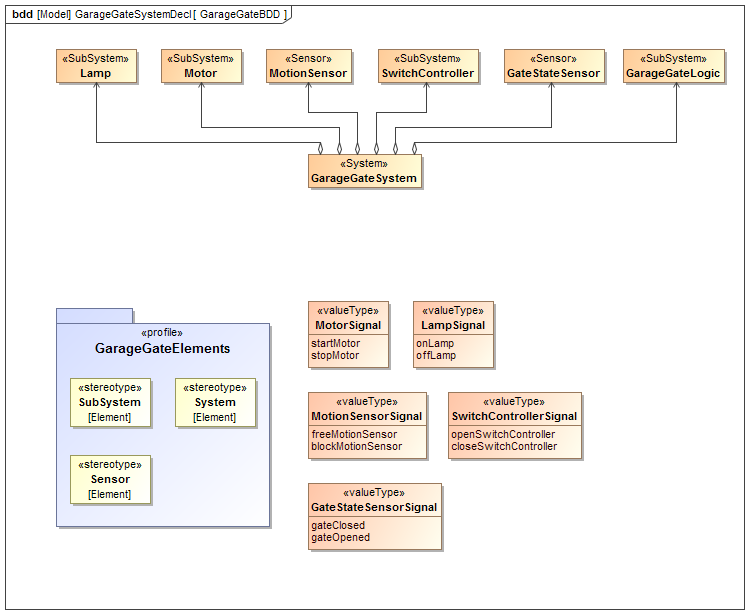
\includegraphics[width=100mm, keepaspectratio]{figures/magicDraw/bdd__GarageGateBDD.png}
	\caption{Garage system components and signals}
	\label{fig:overalBDD}
\end{figure}

First with the control switch we can simply send an action to the control logic that open or close the gate. If someone or something suddenly appears in the way of the gate, while it is moving, the movement stops. The motion sensor detects this interruption (the gate is blocked) or free status (the gate has free way). Before restarting the closing action, the control unit waits 5 seconds for the lighting warning. When the gate is finally closed, an additional sensor gives us plausibility for the gate physically closed state.

%TODO check the requirements
\iffalse
\section{Software Requirements}
\subsection{Gate}
\begin{description}
	\item[Req-01-1] The 
\end{description}
\fi

\subsection{Lamp}
\begin{description}
	\item [REQ-02-1] The lamp lighting frequency should be 1 second.
	\item [REQ-02-2] One lighting section is 5 seconds long.
\end{description}

\subsection{Remote Controller}
\begin{description}
	\item [REQ-03-1] The controller should have an open and a close gate action button.
	\item [REQ-03-2] One action must be completely finished to start a new action. 
	\item [REQ-03-3] When the battery is low, the remote controller should warn this to the control logic. %necessary?
\end{description}

\subsection{Control Logic}
\begin{description}
	\item [REQ-04-1] The \textit{Control Logic} can get new actions from the \textit{Remote Controller}, while no other action is being processed.
	\item [REQ-04-2] While the gates are moving (by an action from the \textit{Remote Controller}), the \textit{Control Logic} should stop the movement, if it gets a \textit{blocking} sign from the \textit{Motion Sensor}. Consequently the \textit{Control Logic} should continue the movement, it it gets a \textit{free} sign from the \textit{Motion Sensor}.
	\item [REQ-04-3] The \textit{Control Logic} can receive the signals from the \textit{Motion Sensor}, \textit{Lamp}, \textit{Remote Controller}
	\item [REQ-04-4] While the \textit{Lamp} is lighting the gates should not move.
\end{description}

\subsection{Motion Sensor}
\begin{description}
	\item [REQ-05-1] The sensor must detect if anything is between the two pillars of the gate. 
	\item [REQ-05-2] If the sensor detect blocking thing in the gate, a \textit{blocking} signal must be sent immediately to the \textit{Control Logic}.
	\item [REQ-05-3] If the sensor can not detect anything between the two gates, a \textit{free} signal must be sent to the \textit{Control Logic}
	\item [REQ-05-4] When the sensor detects free status after the blocking status, there must be at least 3 seconds until the first \textit{free} signal can be sent to the \textit{Control Logic}.
\end{description}

\subsection{Motor}
\begin{description}
	\item [REQ-06-1] 
	\item [REQ-06-2] 
	\item [REQ-06-3] 
\end{description}


%TODO write design details
\section{System model representation}
%specific UML diagrams, component diagram or component composition diagram (like SWSV::RIS description)

First I want to model the physical representation of the sample on the \figref{GarageBDD} figure.

The system consists 5 elements:
\begin{itemize}
	\item Lamp: This component is represents the lamp itself.
	\item Motor: This block can move the gates to opened and closed state.
	\item MotionSensor: These sensors are on the two pillars of the gate, and detect if something is in between of these sensors.
	\item SwitchController: This block is for the remote controller physical realization.
	\item GarStateSensor: The sensor which is detects the actual state of the gate.
    \item GarageGateLogic: This involves the safety logic and the gives control messages to the blocks.
\end{itemize}

\begin{figure}[!ht]
	\centering
	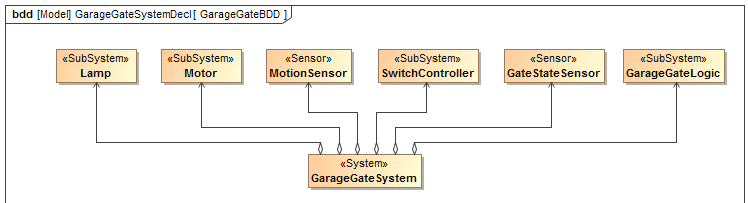
\includegraphics[width=100mm, keepaspectratio]{figures/magicDraw/bdd__GarageGateBDDcut.png}
	\caption{Garage system physical components}
	\label{fig:GarageBDD}
\end{figure}

The \figref{GateLogicComm} figure introduce the communication between the above listed blocks. We can say that each block is connected to one master block, who is the GarageGateLogic with specific ports.

\begin{figure}[!ht]
	\centering
	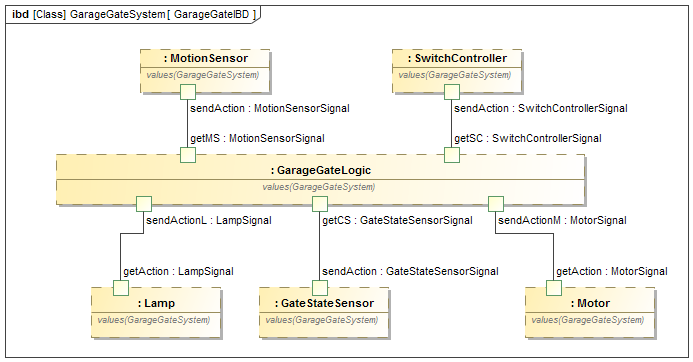
\includegraphics[width=150mm, keepaspectratio]{figures/magicDraw/ibd__GarageGateSystem__GarageGateIBD.png}
	\caption{Gate controller internal block diagram}
	\label{fig:GateLogicComm}
\end{figure}

A garage gate fundamentally have 2 main states, the \textit{Opened} and \textit{Closed} states, which is shown below on \figref{Garage Statemachine} figure. First of all we can start from the initial \textit{Closed} state, where we can open the gate with an 'open' command. This command sets the state machine in an \textit{Opening} state, while starting the motor functions. While opening the gate, somebody or something can move into the way, so this becomes \textit{Block Opening}. The gate is opening again, if the blocking object moved out of the way consequently it is free. After the \textit{Opening} phase succeeded the gate is \textit{Opened}. 

In this state we can 'close' the gate with a simple command by the \textit{Switch Controller}, and the state machine goes to the \textit{Closing} state. There could be also a blocking action, which stops the closing movement. From this state the gate is starting the closing movement again after a few seconds \textit{Lighting}. When the closing action finished the gate is \textit{Closed} and the motor has been stopped.

\begin{figure}[!ht]
\centering
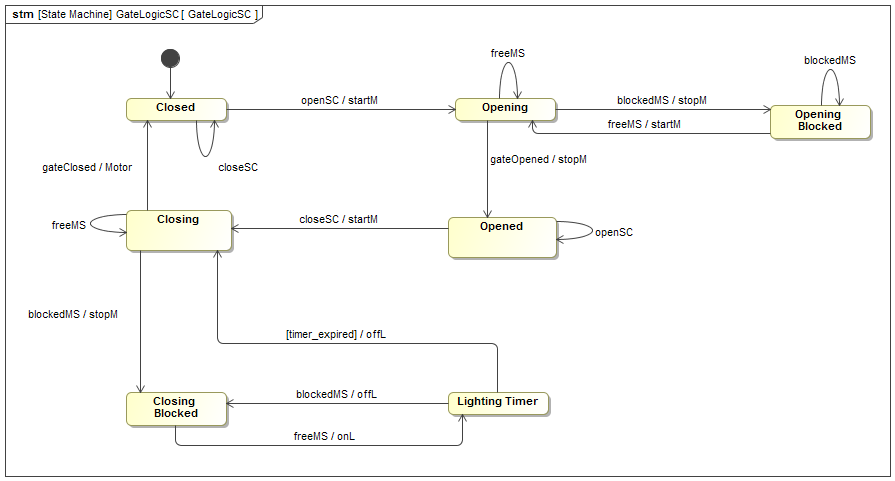
\includegraphics[width=150mm, keepaspectratio]{figures/magicDraw/GateLogicSC.png}
\caption{Garage gate state machine diagram}
\label{fig:Garage Statemachine}
\end{figure}

%TODO define what testing scenarios i will use
\paragraph{Testing goals}
The tests should achieve all the possible states of the SUT, because we want to detect the behaviour of the SUT in all use cases.

\section{Implementation}

\section{Testing results}
\subsection{GraphWalker}

\subsection{SpecExplorer}
%----------------------------------------------------------------------------
\chapter{GraphWalker}\label{sect:GraphWalker implementation of Garage Gate model}

%----------------------------------------------------------------------------
\section{GraphWalker}
%----------------------------------------------------------------------------

\section{GraphWalker implementation in Eclipse}

 We can connect more models with the \textit{SHARED:someName} keyword in a vertex. Consequently I have created a yEd graph model for test scenarios for the garage gate state machine (see \figref{Garage Statemachine}), and a graph model for the lamp, which called from the previous graph.

\begin{figure}[!ht]
	\centering
	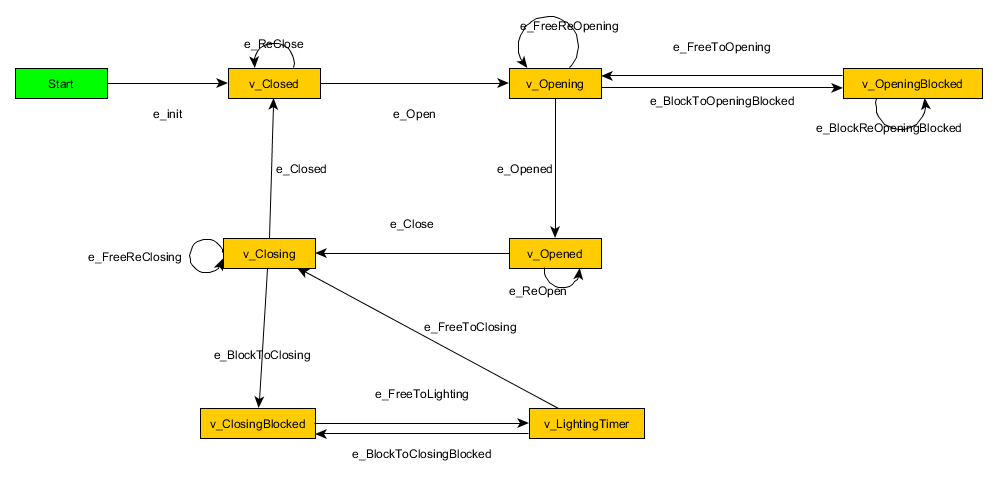
\includegraphics[width=150mm, keepaspectratio]{figures/GateModel.png}
	\caption{Garage gate model with yEd}
	\label{fig:GateModel}
\end{figure}

\begin{figure}[!ht]
	\centering
	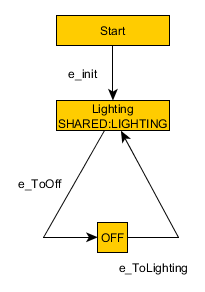
\includegraphics[width=50mm, keepaspectratio]{figures/LightingModel.png}
	\caption{Lamp0 model with yEd}
	\label{fig:LampModel}
\end{figure}


Generated test with option: @GraphWalker(start = "e\_init", value = "random(vertex\_coverage(100))"), and the result was:
[INFO] Result :
[INFO] 
[INFO] {
	"totalFailedNumberOfModels": 0,
	"totalNotExecutedNumberOfModels": 0,
	"totalNumberOfUnvisitedVertices": 0,
	"verticesNotVisited": [],
	"totalNumberOfModels": 2,
	"totalCompletedNumberOfModels": 2,
	"totalNumberOfVisitedEdges": 14,
	"totalIncompleteNumberOfModels": 0,
	"edgesNotVisited": [
	{
		"modelName": "GateModel",
		"edgeId": "e0",
		"edgeName": "e\_init"
	},
	{
		"modelName": "GateModel",
		"edgeId": "e3",
		"edgeName": "e\_Close"
	},
	{
		"modelName": "GateModel",
		"edgeId": "e10",
		"edgeName": "e\_FreeToOpening"
	},
	{
		"modelName": "GateModel",
		"edgeId": "e13",
		"edgeName": "e\_BlockReOpeningBlocked"
	}
	],
	"vertexCoverage": 100,
	"totalNumberOfEdges": 18,
	"totalNumberOfVisitedVertices": 9,
	"edgeCoverage": 77,
	"totalNumberOfVertices": 9,
	"totalNumberOfUnvisitedEdges": 4
}

%TODO implement PyModel stuff
\section{PyModel implementation}
\chapter{Summary}\label{chapt:Summary}
Through the Project Laboratory 2 subject I have tried out two different testing environments and learned a lot about the test execution strategies. I have created a common example project with well-documented specification.
% Acknowledgements, Köszönetnyilvánítás
%~~~~~~~~~~~~~~~~~~~~~~~~~~~~~~~~~~~~~~~~~~~~~~~~~~~~~~~~~~~~~~~~~~~~~~~~~~~~~~~~~~~~~~
%%----------------------------------------------------------------------------
\chapter*{\koszonetnyilvanitas}\addcontentsline{toc}{chapter}{\koszonetnyilvanitas}
%----------------------------------------------------------------------------

Ez nem kötelező, akár törölhető is. Ha a szerző szükségét érzi, itt lehet köszönetet nyilvánítani azoknak, akik hozzájárultak munkájukkal ahhoz, hogy a hallgató a szakdolgozatban vagy diplomamunkában leírt feladatokat sikeresen elvégezze. A konzulensnek való köszönetnyilvánítás sem kötelező, a konzulensnek hivatalosan is dolga, hogy a hallgatót konzultálja.


% List of Figures, Tables
%~~~~~~~~~~~~~~~~~~~~~~~~~~~~~~~~~~~~~~~~~~~~~~~~~~~~~~~~~~~~~~~~~~~~~~~~~~~~~~~~~~~~~~
%\listoffigures\addcontentsline{toc}{chapter}{\abrakjegyzeke}
%\listoftables\addcontentsline{toc}{chapter}{\tablazatokjegyzeke}


% Bibliography
%~~~~~~~~~~~~~~~~~~~~~~~~~~~~~~~~~~~~~~~~~~~~~~~~~~~~~~~~~~~~~~~~~~~~~~~~~~~~~~~~~~~~~~
%\bibliography{bib/mybib}
%\addcontentsline{toc}{chapter}{\irodalomjegyzek}


% Appendix
%~~~~~~~~~~~~~~~~~~~~~~~~~~~~~~~~~~~~~~~~~~~~~~~~~~~~~~~~~~~~~~~~~~~~~~~~~~~~~~~~~~~~~~
%----------------------------------------------------------------------------
\appendix
%----------------------------------------------------------------------------
\chapter*{\fuggelek}\addcontentsline{toc}{chapter}{\fuggelek}
\setcounter{chapter}{\appendixnumber}
%\setcounter{equation}{0} % a fofejezet-szamlalo az angol ABC 6. betuje (F) lesz
\numberwithin{equation}{section}
\numberwithin{figure}{section}
\numberwithin{lstlisting}{section}
%\numberwithin{tabular}{section}


%\label{page:last}
\end{document}
